% RESULTADOS-------------------------------------------------------------------
%Cada capítulo deve conter uma pequena introdução (tipicamente, um ou dois parágrafos) que deve deixar claro o objetivo e o que será discutido no capítulo, bem como a organização do capítulo.
%\chapter{ANÁLISE E DISCUSSÃO DOS RESULTADOS}
\chapter{RESULTADOS}
\label{Chap:Resultados}

Este capítulo apresenta o que foi obtido como resultado deste trabalho e as experiências do autor durante o desenvolvimento do sistema de atualização de firmware over-the-air. Primeiro será apresentado os resultados mostrando como é um processo de atualização realizado com sucesso e em seguida discutido o uso e vantagens e desvantagens do sistema. 
Inicialmente irei falar sobre qual o firmware que foi gerado para este teste, seu conteúdo e suas variáveis que fariam a diferenciação entre os as versões de firmwares, e mostrando as etapas em de atualização que são realizadas neste processo.

\section {FIRMWARES DE TESTE PROPOSTOS}
Para os testes apresentados neste trabalho foram desenvolvidos três firmwares muito parecidos, ambos possuem todas as bibliotecas necessárias para que sistema de atualização OTA proposto funcionem corretamente, além de possuírem o sistema operacional de tempo real FreeRTOS. Esses firmwares foram desenvolvido para somente darem suporte ao sistema e não exercerem nenhuma outra função, então temos uma estimativa do tamanho que somente o sistema de atualização, suas bibliotecas e o FreeRTOS ocupam em memória.

Esses firmwares contém em sua função main, além de inicializações necessárias de drivers, bibliotecas e do sistema operacional, uma pequena função que apresenta uma mensagem de apresentação mostrando a versão do firmware atual e uma mensagem de teste somente para fazer uma diferenciação entre as versões e como mostrada na \autoref{mensagemteste}. 

\begin{figure}[H]
    \scriptsize
     \centering
     
\includegraphics[scale=1.2]{dados/figuras/ToDo.jpg}
     \caption{As três mensagens exibidas para diferenciação dos \firmware. \newline Fonte: Autoria própria.}
     \label{mensagemteste}
\end{figure}

A função padrão destes firmware é um laço infinito que a cada XXXX segundos inicializa a função OTA que inicializa o processo de atualização, assim temos uma garantia que o firmware ira sempre ficar executando a funçao OTA.

\section{PROCESSO DE ATUALIZAÇÃO DE FIRMWARE}
Aqui apresentaremos todo o processo de atualização feito para assim comprovar o funcionamento do sistema desenvolvido neste trabalho, com isso é abordado desde a inicialização do firmware que será substituído, a disponibilização de um novo firmware no servidor, a inicialização deste firmware na plataforma embarcada STM32F746G e sua mensagem de apresentação.

\subsection{ESTADO INICIAL DO MICROCONTROLADOR}
Inicialmente é gravado no microcontrolador o bootloader e depois o firmware 1, com isso temos a memória FLASH preenchida separadamente, visto que definimos areas diferentes para aplicação e bootloader no arquivo de linker, assim fica o estado inicial da memória do microcontrolador no inicio do teste.

Com o bootloader e firmware 1 gravados no hardware já é possivel fazer a primeira inicialização do sistema, com a reinicialização do hardware o sistema inicializa o bootloader para poder dar sequencia de atualização ou pulo para a aplicação.

\subsection{INICIALIZAÇÃO DO BOOTLOADER}
Após todos processos de inicialização o bootloader é executado, como o intuito é que ele seja pequeno e de forma que se adapte para todos os tipos de microcontroladores da familia STM32, não existe nenhum tipo de sinalização durante seus processos, assim sua função principal que é fazer a troca de firmware e pulo para a aplicação é executada de forma que o usuário não é capas de identificar.

Durante sua execução o bootloader checa a versão do firmware atual e o compara com a versão que está no cartão SD, caso a versão atual for menor ou não seja encontra a nova versão do firmware o bootloader inicializa o firmware que está na memória flash. Como neste caso de teste o cartão SD se encontra vazio, o bootloader assume que não há nenhuma atualização a ser efetuada, assim ele inicializa a sequência de pulo para a aplicação. 
\subsection{INICIALIZAÇÃO DO FIRMWARE 1}
Com a inicialização a aplicação efetuada pelo bootloader, são executadas todas as inicializações de drivers, das bibliotecas utilizadas pelo firmware 1, e assim inicializado o sistema operacional FreeRTOS, e exibida via UART a mensagem de confirmação de montagem do driver do cartão SD e a mensagem de apresentação contendo a versão do software atual e o sua frase de identificação como pode ser observado na \autoref{fraseidentificacao}. A partir da impressão dessa frase o sistema operacional iniciará a tarefa OTA.

\begin{figure}[H]
    \scriptsize
     \centering
     
\includegraphics[scale=1.2]{dados/figuras/ToDo.jpg}
     \caption{As três mensagens exibidas para diferenciação dos \firmware. \newline Fonte: Autoria própria.}
     \label{fraseidentificacao}
\end{figure}


\subsection{OTA}
Ao iniciar a função OTA será buscado no servidor o arquivo contendo a versão do firmware 2, com esse arquivo baixado ele fará a comparação com a versão atual do firmware e caso necessário irá fazer o download do novo firmware, e do arquivo contendo o hash deste firmware, tendo esses arquivos salvos no cartão SD ele ira fazer o hash do firmware baixado e verificar assim a integridade do arquivo baixado. Caso todos os processos ocorram com sucesso ele irá fazer com que esses arquivos permaneçam no cartão SD e iniciará o processo de pulo para o bootloader, que encerra todos os driver e o sistema operacional e pula para a região do bootloader para o executar. Todo esse processo pode ser visto na \autoref{processoOTA}.

\begin{figure}[H]
    \scriptsize
     \centering
     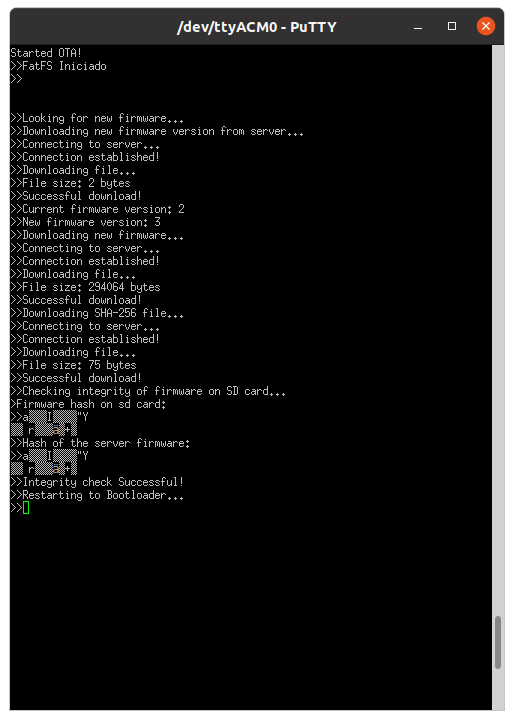
\includegraphics[scale=0.7]{dados/figuras/atualizaçãoOTAcompleto.png}
     \caption{Processo de atualização OTA. \newline Fonte: Autoria própria.}
     \label{processoOTA}
\end{figure}

\subsection{REINICIALIZAÇÃO DO SISTEMA PARA O BOOTLOADER}
O bootloader é inicializado novamente, mas agora ele consegue achar um arquivo de versão escrito no cartão SD e com isso fazer a comparação com a versão de firmware e como a versão encontrada no cartão SD é maior que a escrita na flash ele iniciará o processo de troca de firmware.
Após a troca de firmware ele escreverá na ultima posição da memória a versão do novo firmware, fazendo com que atualização seja concluída com sucesso, assim podendo novamente fazer o processo de pulo para a aplicação.
\subsection{INICIALIZAÇÃO DO FIRMWARE 2}
Após o pulo para aplicação efetuada pelo bootloader após a atualização são executadas todas as inicializações de drivers, das bibliotecas utilizadas pelo firmware 2, e assim inicializado o sistema operacional, exibida a mensagem de confirmação de montagem do driver do cartão SD e a mensagem de apresentação contendo a versão do software atual e o sua nova frase de identificação como pode ser observado na \autoref{fraseidentificacao2}. Assim concluindo com sucesso um processo de atualização de firmware.

\begin{figure}[H]
    \scriptsize
     \centering
     
\includegraphics[scale=1.2]{dados/figuras/ToDo.jpg}
     \caption{As três mensagens exibidas para diferenciação dos \firmware. \newline Fonte: Autoria própria.}
     \label{fraseidentificacao2}
\end{figure}



\section{DISCUSSÃO}
Os resultado obtidos mostraram que o sistema de atualização de firmware Over-The-Air proposto neste trabalho funciona, e que todo o processo desde a verificação de uma aplicação integra feita pelo bootloader, seu processo de atualização e as verificações, obtenções e verificações de arquivos da API de atualização OTA ocorrem com sucesso.

Como o bootloader ocupa XX Kbytes de espaço na memória FLASH ele pode ser utilizado por diversas placas da familia de microcontroladores STM32 que possuam um setor da memória maior que esse espaço. Com a aplicação que foi utilizada para testar este trabalho que possui em seu código somente a API de atualização, as bibliotecas que são necessárias para este trabalho e o sistema operacional FreeRTOS ocupam juntos cerca de 294 Kbytes, a aplicação do usuário ainda teria um espaço de 674 Kbytes restante na plataforma que utilizamos para teste se contarmos junto o espaço reservado para o bootloader. Esta aplicação ainda não precisaria incluir novamente as bibliotecas FATFS, MBED TLS, LWIP e o sistema operacional FreeRTOS. 

Com essa informação sobre o tamanho dos arquivos, é possível notar que este sistema de atualização não é tão portável quanto se esperava no inicio deste trabalho, visto que só para ter um sistema de atualização funcional precisamos que o hardware em que se deseja ter esse sistema tenha ao menos 512 Kbytes de memória FLASH, diminuindo muito a quantidade de microcontroladores que poderiam utilizar este sistema.

Ainda assim é possível afirmar que o sistema cumpre com o objetivo geral e específicos propostos, visto que o sistema é capaz de efetuar a atualização da plataforma embarcada STM32F746NGH6 da forma proposta e ainda é capaz de identificar quando houve falhas em seu sistema de atualização e se recuperar de forma autónoma dessas falhas.
